\documentclass[tikz,border=8pt]{standalone}
% Shared look for every TikZ diagram. Load with \input{../../tools/tikz-style.tex}
\usepackage[sfdefault]{roboto}
\usetikzlibrary{arrows.meta, positioning, shapes.geometric, calc, fit, backgrounds}
\definecolor{cblue}{HTML}{4C78A8}
\definecolor{corange}{HTML}{F58518}
\definecolor{cgreen}{HTML}{54A24B}
\definecolor{cred}{HTML}{E45756}
\definecolor{cpurple}{HTML}{B279A2}
\definecolor{cgrey}{HTML}{6B6B6B}
\tikzset{
  every picture/.style={font=\sffamily, line width=1.2pt},
  box/.style={draw=#1, fill=#1!12, rounded corners=4pt, align=center, inner sep=7pt, minimum height=1.1cm},
  box/.default=cgrey,
  arrow/.style={-{Stealth[length=3mm]}, draw=cgrey, line width=1.4pt},
  title/.style={font=\sffamily\bfseries\Large},
  note/.style={font=\sffamily\small, text=cgrey, align=center},
}
\AtBeginDocument{\hyphenpenalty=10000 \exhyphenpenalty=10000}

% The error in the robot's own frame (Kanayama et al. 1991, eq. 3), drawn 20 cm per metre.
% (a) robot facing 0 deg, timetable point 0.2 m further along x and 0.1 m lower: x_e = 0.2, y_e = -0.1.
% (b) the same world offset, robot facing 45 deg: x_e = 0.0707, y_e = -0.2121.
% (c) the error of Section 5.2's check: x_e = 0.2, y_e = -0.1, the timetable's heading 30 deg left of the robot's.
\begin{document}
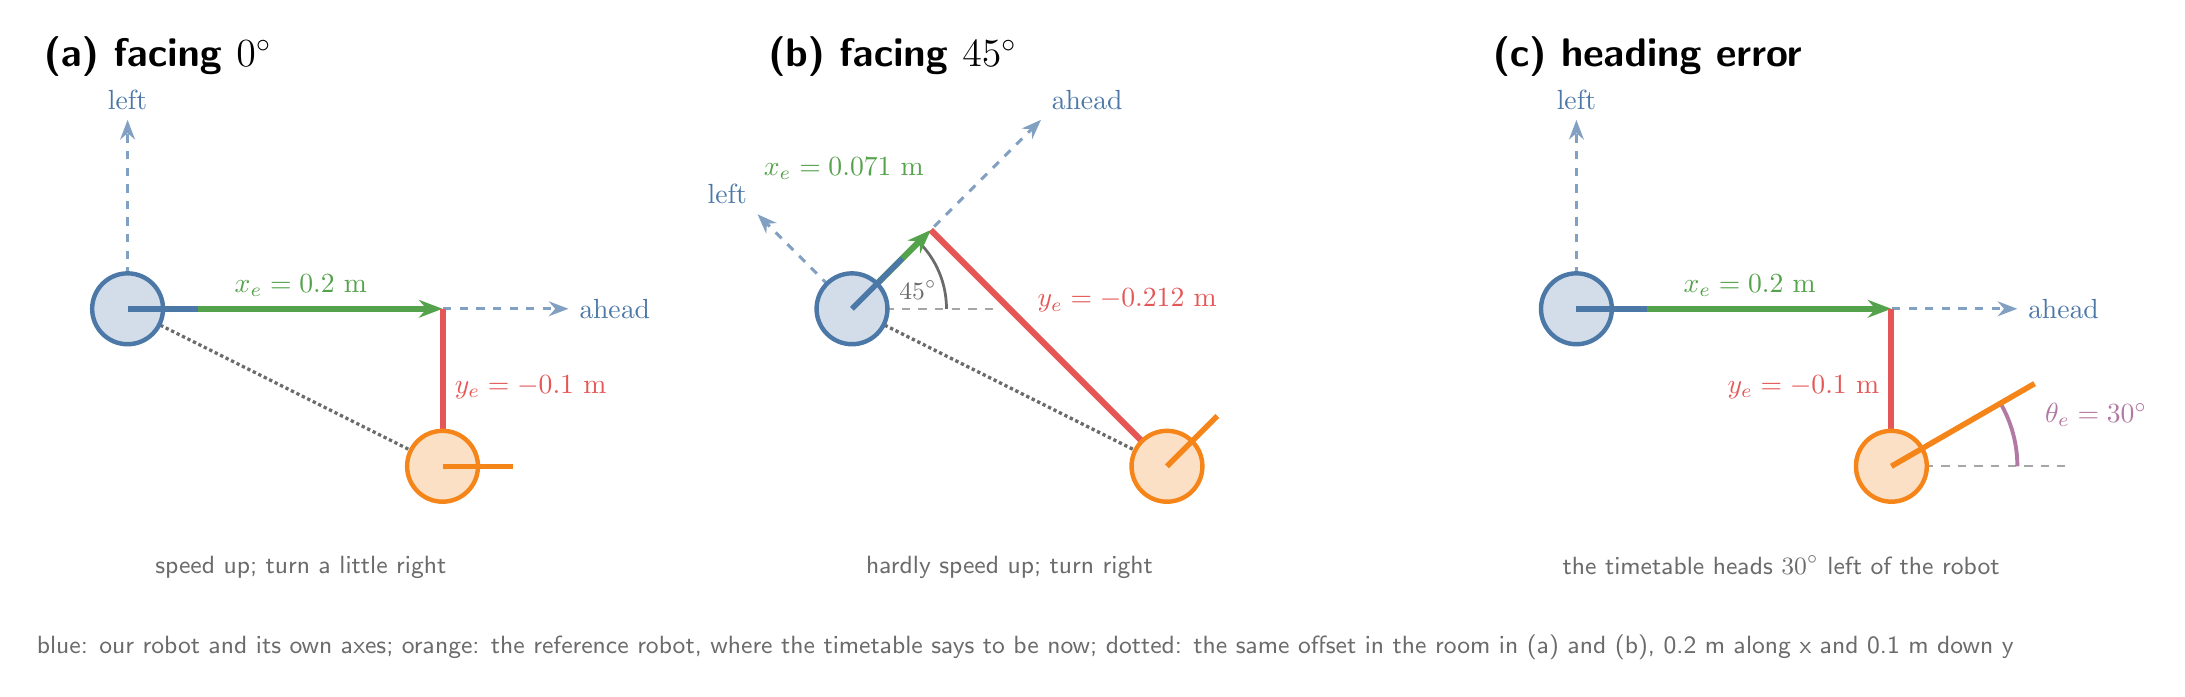
\begin{tikzpicture}[every node/.append style={font=\normalsize},
  rob/.style={draw=#1, fill=#1!25, line width=1.6pt},
  ax/.style={-{Stealth[length=2.5mm]}, draw=cblue!70, line width=1.1pt, dashed},
  err/.style={-{Stealth[length=3mm]}, line width=2.2pt}]
  % ---------- (a) ----------
  \begin{scope}
    \node[title, anchor=west] at (-1.2,3.2) {(a) facing $0^\circ$};
    \draw[ax] (0,0) -- (5.6,0) node[right, text=cblue] {ahead};
    \draw[ax] (0,0) -- (0,2.4) node[above, text=cblue] {left};
    \draw[cgrey, line width=1.2pt, -{Stealth[length=2.5mm]}, densely dotted] (0,0) -- (4,-2);
    \draw[err, cgreen] (0,0) -- node[above, pos=0.55] {$x_e = 0.2$ m} (4,0);
    \draw[err, cred] (4,0) -- node[right] {$y_e = -0.1$ m} (4,-2);
    \draw[rob=cblue] (0,0) circle (0.45); \draw[cblue, line width=2pt] (0,0) -- (0.9,0);
    \draw[rob=corange] (4,-2) circle (0.45); \draw[corange, line width=2pt] (4,-2) -- (4.9,-2);
    \node[note, anchor=north] at (2.2,-3.0) {speed up; turn a little right};
  \end{scope}
  % ---------- (b) ----------
  \begin{scope}[xshift=9.2cm]
    \node[title, anchor=west] at (-1.2,3.2) {(b) facing $45^\circ$};
    \draw[ax] (0,0) -- (2.4,2.4) node[above right, text=cblue] {ahead};
    \draw[ax] (0,0) -- (-1.2,1.2) node[above left, text=cblue] {left};
    \draw[cgrey!60, line width=0.8pt, dashed] (0,0) -- (1.8,0);
    \draw[cgrey, line width=1pt] (1.2,0) arc (0:45:1.2); \node[cgrey, font=\small] at (0.84,0.24) {$45^\circ$};
    \draw[cgrey, line width=1.2pt, -{Stealth[length=2.5mm]}, densely dotted] (0,0) -- (4,-2);
    \draw[err, cgreen] (0,0) -- (1,1); \node[cgreen, anchor=south east] at (1.05,1.5) {$x_e = 0.071$ m};
    \draw[err, cred] (1,1) -- node[above right, pos=0.4] {$y_e = -0.212$ m} (4,-2);
    \draw[rob=cblue] (0,0) circle (0.45); \draw[cblue, line width=2pt] (0,0) -- (0.64,0.64);
    \draw[rob=corange] (4,-2) circle (0.45); \draw[corange, line width=2pt] (4,-2) -- (4.64,-1.36);
    \node[note, anchor=north] at (2.0,-3.0) {hardly speed up; turn right};
  \end{scope}
  % ---------- (c) ----------
  \begin{scope}[xshift=18.4cm]
    \node[title, anchor=west] at (-1.2,3.2) {(c) heading error};
    \draw[ax] (0,0) -- (5.6,0) node[right, text=cblue] {ahead};
    \draw[ax] (0,0) -- (0,2.4) node[above, text=cblue] {left};
    \draw[err, cgreen] (0,0) -- node[above, pos=0.55] {$x_e = 0.2$ m} (4,0);
    \draw[err, cred] (4,0) -- node[left] {$y_e = -0.1$ m} (4,-2);
    \draw[cgrey!60, line width=0.8pt, dashed] (4,-2) -- (6.2,-2);
    \draw[cpurple, line width=1.4pt] (5.6,-2) arc (0:30:1.6); \node[cpurple] at (6.6,-1.35) {$\theta_e = 30^\circ$};
    \draw[rob=cblue] (0,0) circle (0.45); \draw[cblue, line width=2pt] (0,0) -- (0.9,0);
    \draw[rob=corange] (4,-2) circle (0.45); \draw[corange, line width=2pt] (4,-2) -- ++(30:2.1);
    \node[note, anchor=north] at (2.6,-3.0) {the timetable heads $30^\circ$ left of the robot};
  \end{scope}
  \node[note, anchor=north] at (11.4,-4.0) {blue: our robot and its own axes; orange: the reference robot, where the timetable says to be now; dotted: the same offset in the room in (a) and (b), 0.2 m along x and 0.1 m down y};
\end{tikzpicture}
\end{document}
